\documentclass[a4paper,12pt,twoside]{report}

\usepackage[T1]{fontenc} \usepackage{lmodern} \usepackage[utf8]{inputenc}
\usepackage[english]{babel} \usepackage{csquotes}
\usepackage{float} \usepackage{graphicx,subfig}
\usepackage{amssymb,amsmath} \usepackage{siunitx}
\usepackage[style=numeric,backend=biber]{biblatex} \bibliography{refs}
\usepackage[top=4cm,bottom=4cm,left=3cm,right=3cm,headheight=15pt]{geometry}
\usepackage{fancyhdr} \pagestyle{fancy} \usepackage{lastpage}
%\usepackage{parskip} \setlength{\parindent}{0em} \setlength{\parskip}{1em}
\usepackage[colorlinks=true,allcolors=blue]{hyperref} \hypersetup{
	pdfauthor={Michaël Defferrard},
	pdftitle={Audio Classification with Structured Deep Learning},
	pdfsubject={Master project in Information Technologies}
}

\lhead{Audio Classification with Structured Deep Learning} \chead{} \rhead{}
\cfoot{\thepage / \pageref{LastPage}}

\usepackage[acronym]{glossaries} \makeglossaries
\newacronym{EPFL}{EPFL}{École Polytechnique Fédérale de Lausanne}
\newacronym{ICASSP}{ICASSP}{International Conference on Acoustics, Speech and Signal Processing}
\newacronym{MIR}{MIR}{Music Information Retrieval}
\newacronym{MGR}{MGR}{Music Genre Recognition}
\newacronym{PSD}{PSD}{Predictive Sparse Decomposition}
\newacronym{CQT}{CQT}{Constant-Q Transform}
\newacronym{LCN}{LCN}{Local Contrast Normalization}
\newacronym{SVM}{SVM}{Support Vector Machine}
\newacronym{RIP}{RIP}{Restricted Isometry Property}
\newacronym{BP}{BP}{Basis Pursuit}
\newacronym{FISTA}{FISTA}{Fast Iterative Shrinkage-Thresholding Algorithm}
\newacronym{ADMM}{ADMM}{Alternating Direction Method of Multipliers}
\newacronym{PD}{PD}{Primal-Dual}
\newacronym{SGD}{SGD}{Stochastic Gradient Descent}
\newacronym{GPU}{GPU}{Graphical Processing Unit}
\newacronym{LASSO}{LASSO}{Least Absolute Shrinkage and Selection Operator}
\newacronym{AGC}{AGC}{Automatic Gain Control}
\newacronym{kNN}{kNN}{k Nearest Neighbors}

\newcommand{\eqnref}[1]{(\ref{#1})}  % Eqn~(\ref{#1})
\newcommand{\figref}[1]{Figure~\ref{#1}}
\newcommand{\tabref}[1]{Table~\ref{#1}}
\newcommand{\HRule}{\rule{\linewidth}{0.5mm}}

\newcommand{\R}{\mathbb{R}}
\DeclareMathOperator*{\argminop}{arg\,min}
\DeclareMathOperator*{\sgn}{sgn}
\DeclareMathOperator*{\tr}{tr}
\newcommand{\argmin}[1]{\argminop\limits_{#1}}
\newcommand{\minimize}[1]{\min\limits_{#1}}
\newcommand{\normT}[1]{\| #1 \|_2^2}
\newcommand{\normO}[1]{\| #1 \|_1}
\newcommand{\normZ}[1]{\| #1 \|_0}
\newcommand{\normF}[1]{\| #1 \|_\text{F}^2}
\newcommand{\inner}[2]{\langle #1 , #2 \rangle}
\renewcommand{\L}{\mathbf{L}}
\newcommand{\D}{\mathbf{D}}
\newcommand{\E}{\mathbf{E}}
\newcommand{\X}{\mathbf{X}}
\newcommand{\Z}{\mathbf{Z}}
\renewcommand{\d}{\mathbf{d}}
\newcommand{\e}{\mathbf{e}}
\newcommand{\x}{\mathbf{x}}
\newcommand{\y}{\mathbf{y}}
\newcommand{\z}{\mathbf{z}}
\newcommand{\Eone}{E_1(\Z, \D)}
\newcommand{\Etwo}{E_2(\Z, \D, \E)}
\newcommand{\Ethree}{E_3(\Z, \D, \E)}
\newcommand{\G}{\mathcal{G}}
\newcommand{\set}[2]{\{#1_i\}_{i=1}^#2}
\newcommand{\st}{\text{ s.t. }}
\newcommand{\cst}[2]{\|#1_#2\|_2 \leq 1}
%\newcommand{\forallx}[2]{\forall #1 \in \{1,\ldots,#2\}}
\newcommand{\forallx}[2]{#1 = 1, \ldots, #2}
%\newcommand{\forallx}[2]{\|#1_#2\|_2 \leq 1 \text{ for } #2 = 1,\ldots,#3}
\newcommand{\cstd}{\cst{\d}{i}, \forallx{i}{m}}
\newcommand{\cste}{\cst{\e}{k}, \forallx{k}{n}}
\newcommand{\pd}[2]{\frac{\partial #1}{\partial #2}}

\begin{document}

\hypersetup{pageanchor=false}
\begin{titlepage}
	
	
\includegraphics[height=2.5cm]{img/logo_epfl}
	\hfill
	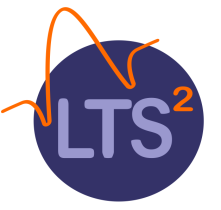
\includegraphics[height=2.5cm]{img/logo_lts2}
	\vspace{1.5cm}
	
	\begin{center}
		
		\textsc{\LARGE MASTER THESIS}\\
		\vspace{0.5cm}
		\large Electrical and Electronic Section\\
		\large Major in Information Technologies\\
		\vspace{1.3cm}
		
		\HRule
		\vspace{1.0cm}
		\textsc{\Huge Audio Classification with}\\
		\vspace{0.7cm}
		\textsc{\Huge Structured Deep Learning}\\
		\vspace{0.6cm}
		\HRule
		\vspace{1.3cm}
		
		\begin{minipage}{0.45\textwidth}
			\begin{flushleft} \large
				\textbf{Student}\\ \vspace{0.5ex}
				Michaël \textsc{Defferrard} \\ \vspace{2.5ex}
				\textbf{Professor} \\ \vspace{0.5ex}
				Pierre \textsc{Vandergheynst}
			\end{flushleft}
		\end{minipage}
		\begin{minipage}{0.45\textwidth}
			\begin{flushright} \large
				\textbf{Supervisors} \\ \vspace{0.5ex}
				Xavier \textsc{Bresson} \\ \vspace{0.2ex}
				Johan \textsc{Paratte}
			\end{flushright}
		\end{minipage}
		
	\end{center}
	
	\vspace{1.3cm}
	{\large Conducted at the EPFL LTS2 laboratory.}
	\vspace{1.3cm}

	\begin{center}
		{\large June 19, 2015}
	\end{center}
	
\end{titlepage}
\hypersetup{pageanchor=true}

\begin{abstract}
	In this work, we present a technique to learn discriminative audio features for \gls{MIR} in an unsupervised and hierarchical way. We introduce a novel deep architecture composed by (stacks of) structured sparse auto-encoders which leverage on the recent advances of deep learning using efficient auto-encoder strategy that simultaneously learned sparse representation of inputs and dictionary adapted to those inputs. Our main goal is to find a solution to sparse coding that is structured by the proximities of the sparse features encoded by a graph of audio inputs. We borrow ideas from manifold learning to constrain our solution to be smooth on this graph, i.e. to have a small Dirichlet energy, in order to implicitly force feature proximities. Our auto-encoder model is formulated as a non-convex optimization problem, for which a {\color{red}well-posed} iterative scheme is provided. We show that the learned features combined with a simple linear classifier achieve {\color{red}110\%} accuracy in predicting genres on GTZAN.
\end{abstract}

\renewcommand{\abstractname}{Acknowledgements}
\begin{abstract}
	Xavier for day-to-day supervision. Many inputs and intuitions. Discussion of the results.
	
	Johan for intuitions at the start of the project, advices and proof reading of the thesis.
	
	Pierre
	%C’est grâce à vous que je suis satisfait de conclure ce travail éternellement inachevé par cette petite note personnelle dans une langue que je chéris beaucoup.
	
\end{abstract}

%\clearpage
%\setcounter{page}{2}
\tableofcontents

\printglossaries
\addcontentsline{toc}{chapter}{Glossary}
\addcontentsline{toc}{chapter}{Acronyms}

\chapter*{Introduction}
\addcontentsline{toc}{chapter}{Introduction}

This work was accomplished as a Master thesis, which is an integral part of the major in Information Technologies curriculum from the Electrical and Electronic Section of the \gls{EPFL}. It was conducted at the LTS2 laboratory\footnote{The laboratory homepage is accessible at \url{http://lts2www.epfl.ch/}.}.

While the project was ongoing, I continuously published my thoughts, observations, findings, experiments, results and plans as well as a summary of the weekly meetings with my supervisors on an online blog\footnote{My research blog is available at \url{https://lts2research.epfl.ch/blog/mdeff/}.} in the format of an open laboratory notebook\footnote{\url{http://en.wikipedia.org/wiki/Open_notebook_science}}. The code, as well as the results, this report and the ongoing paper is versioned with git and available online through GitHub\footnote{My GitHub account can be found at \url{https://github.com/mdeff}.}. A continuation of this work shall be submitted to the 41st IEEE \gls{ICASSP}.

\section*{Motivation}
\addcontentsline{toc}{section}{Motivation}

\section*{Background}
\addcontentsline{toc}{section}{Background}
\label{background}

\section*{Related work}
\addcontentsline{toc}{section}{Related work}
% LeCun's paper

\part{Theoretical foundations}
% Explain the methods we'll later use.

\chapter{Music theory}
% Explain how music is constructed.

\section{Notes and frequencies}

\section{Harmonics, chords and harmonies}

\section{Constant-Q transform}
% Spectrogram with geometrically spaced frequencies.

\section{Genres}
% How we can qualitatively distinguish genres.

\chapter{Machine learning}
% What's the purpose of learning.
% Why learned features instead of hand-crafted features ?

\section{Supervised vs unsupervised}
% Explain the difference. Why do we want unsupervised ?

\section{Feature / representation learning}
% NN is well suited for representation learning
% We want unsupervised feature learning vs supervised vs hand-crafted

\section{Support Vector Machine}
% Used for classification

\section{Neural networks}
% Why ? Distributed representation and computation (e.g. training on GPU, clusters) --> much what symbolic AI is not (mainly search algorithms, SAT solvers)
% Started in the late 1950s with the perceptron.

\subsection{Deep learning}
% Rebranded as deep learning, achieve now astonishing results in a variety of fields (computer vision, NLP, machine translation, knowledge representation, automatic control)
% Deep learning: hierarchical feature learning --> we are not really using that (yet)
% Deep architectures can approximate any function (RNN any program, i.e. Turing complete)
% First fall of NN (success of kernel methods / SVM) (first AI winter ?) because perceptron was proved to not be sufficient, multi-layer was too hard (computation and training)
% Computationally expensive to train
% Needed to invent backpropagation to train multiple layers
% Hard to train: problem of vanishing gradient
% Objective function is highly non-convex.

\section{Sparse coding}
% What it is, why it works, why it's good.
% Why learning a dictionary.
% paper who demonstrates that L1 penalty leads to same solution as L0 while being convex, not combinatorial

\subsection{Dictionary learning}
% under-complete: dimensionality reduction, no solution to x = Dz.
% over-complete: easier (linear) separability in higher dimensional space (number of dictionary elements is larger than the dimension of the input data). Infinitely many solutions to x = Dz, need prior and optim to find the 'best' (simplest, l1 norm) one.
% overcompleteness must be evaluated by considering the number of code units and the effective dimensionality of the input as given by PCA
% the representation is exploiting statistical regularities present in the training set

\subsection{Encoder}
% Problem: these methods are slow at inferring sparse codes as they need iterations
% --> train an encoder

\section{Auto-encoders}
% For unsupervised learning, i.e. feature extraction.
% Auto-encoders as a manifold learning tool (Bengio review).

\subsection{Sparse auto-encoders}

\subsection{Denoising auto-encoders}
% Compare with denoising auto-encoders

\chapter{Convex optimization}

\section{Convex problem}
% What is a convex problem (objective and constraints).
% Methods to solve: analytically or numerical schemes.

\section{Numerical solvers}
% Numerical: gradient descent --> slow --> second order methods like Newton
% Stochastic gradient descent

\section{Proximal splitting methods}
% But our objective function is not differentiable
% --> rely on a sub-gradient method, the proximity / proximal operator --> proximal splitting

\subsection{Forward-backward}
% Different basic methods to solve these problems: forward-backward, douglas-rachford
% Explain the intuition

\subsection{Douglas-Rachford}

\subsection{FISTA}
% Advanced (faster) algorithms who exlpoit variable time steps and multiple points: FISTA

\section{Dual problem}
% Introducing the dual problem (paper playing with duality)

\subsection{Primal-dual}

\chapter{Spectral graph theory}
% Paper: Pierre's review

\section{Manifold}
% The graph is a discrete approximation of the unknown manifold. We sample the manifold.

\section{Graph}
% What is a graph --> discrete approximation of a low-dimensional manifold embedded in a high dimensional space.
% Type of graph (KNN vs epsilon), kernel (Gaussian, polynomial), distance (Euclidean, cosine)

\subsection{Approximate KNN search}
% How FLANN works, what are the alternatives.
% Techniques: KDtree, ball, local hashes (LHS)

\subsection{Distance metric}
% euclidean (small dim) and cosine (angular, high dim)

\subsection{Kernel}
% Gaussian or polynomial

\section{Spectrum}
% What does the spectrum / Fourier transform mean: examples on a 3D point cloud.
% Faster way to compute FT: Chebyshev approximation (filter bank)

\section{Laplacian}
% The graph Laplacian is an approximation of the Laplace-Beltrami operator. --> Dirichlet energy
% normalized vs un-normalized, cite normalized approximates the Laplace-Beltrami operator
% A way to test if the Laplacian is well constructed is... (see blog)

\part{Contributions}
\label{contributions}
% Proposed method / method
% Based on the introduced methods, explain what we did.

\chapter{Model}
% Visual diagram

\section{Hypothesis}

% (Known) hypothesis: patches of spectrogram are composed by a linear combination of atoms. These atoms form a dictionary. As we shall see, these atoms represent harmonies, harmonics, drums etc.

% (New) hypothesis: audio spectrograms lie on a low-dimensional manifold embedded in a high dimensional space.
% Structured: adding similarity information between inputs
% Manifold: not all possible signals are reasonable / feasible

% Finish with the complete objective function.
% Why energy function ? Many laws of nature are nothing but optimality conditions, often expressed in terms of a minimum energy principle.
% Easy to add and remove terms.

\section{Graph construction}
% Similarity measure
% KNN graph

\section{Problem formulation}
% Construction: sparse coding, dictionary learning, encoder learning, manifold learning
% Non-convex problem composed of convex sub-problems.
% Derive prox and gradients.
% Why we can use FISTA an PD ?
% Derive FISTA and primal-dual formulations.

\section{Training}
% Batch (FISTA, primal-dual) and online (stochastic gradient descent) training
% Transductive learning

\section{Feature extraction}
% Most accurate extraction with original model.
% Much faster approximations by ignoring some terms of the objective.

\section{Audio pre-processing}
% Frames, CQT, LCN, feature / sample normalization

\section{Classification}
% Feature aggregation (feature vectors), linear SVM, majority voting (winner take all)
% Voting further gives a cheap confidence level about our choice.
% Multi-class: one-vs-one / one-vs-the-rest

\chapter{Implementation}

\section{Framework}
% Stack: numpy, scipy, matplotlib, scikit-learn, librosa
% Tools: IPython notebook, CDK cluster, matplotlib, h5py, librosa
% Explain why and how data is stored (layout) via HDF5.

\subsection{PyUNLocBoX}
% PyUNLocBoX: explains how it works

\section{Design}

\section{Performance}

\subsection{Algorithm}
% FISTA vs PD implementation

\subsection{Optimization for space}
% Optimization for space: avoid copy, modify in place, float32, store Z as scipy.sparse

\subsection{Optimization for speed}
% Optimization for speed: ATLAS/OpenBLAS, float32 (memory bandwidth), projection in the ball (not on the sphere)
% ATLAS mono-threaded (at least on Ubuntu), OpenBLAS multi-threaded.
% Linear algebra: optimized version of BLAS: ATLAS and OpenBLAS. (LINPACK)

\chapter{Results}
\label{results}
% Results and comparisons
% Include discussion in results ?

\section{Spectrograms}
% Show example spectrograms of jazz / blues. Show how they are different (music theory) and can such be distinguished.

\section{Learned features}
% Show some atoms: harmonics, chords, harmonies, drums.
% Probably not on full CQT, should be on octaves.

\section{Descriptive feature vectors}
% Show aggregated feature vectors for some genres.
% How is it qualitatively more discriminative than the spectrogram ?

\section{Hyper-parameters tuning}
% Test matrix for hyper-parameters on smaller problem (i.e. less frames).
% For ld, le, lg, m
% Numerical parameters: Nouter (enough when no more inner), rtol
% Graph parameters: K, Csigma, kernel?, metric
% Classification: C, Nvectors
% Pre-processing: na=1024, ns=96

\section{Classification accuracy}
% Measured via 10-fold cross-validation
% How classification is improved by feature learning, introducing the encoder / graph.
% Comparison with other techniques.

\chapter{Discussion}
\label{discussion}
% Discussion of our results. Strengths and weaknesses of our method.

\chapter*{Conclusion}
\addcontentsline{toc}{chapter}{Conclusion}
\label{conclusion}

\section*{Future work}
\addcontentsline{toc}{section}{Future work}

\paragraph{Encoder}

\paragraph{LCN}
% Not if we cannot justify.

\paragraph{Individual octaves}

\paragraph{TV norm}
% TV norm on the graph instead of Dirichlet energy

\paragraph{Distributed implementation}
% Train chunks of D / Z via independant threads.
% Directly in the PyUNLocBoX ?
% Usefull only if we are not memory bandwidth limited.
% Why ATLAS does not do it by default ? OpenBLAS does it.
% Move to GPU.

\paragraph{Multiple layers}
% Multiple layers of auto-encoders

\paragraph{End-to-end learning}
% Learn features right from raw audio. If spectrograms are good features, we should retrieve them.

\paragraph{Domain knowledge}
% Incorporate some domain knowledge about the dictionary via priors. Then it's not supervised anymore.
% Priors on the dictionary who are not necessarily domain specific, i.e. are general enough to apply to other kind of data.

\printbibliography
\addcontentsline{toc}{chapter}{References}

\chapter*{Annexes}
\addcontentsline{toc}{chapter}{Annexes}
\label{annexes}

\section*{Conference paper}
\addcontentsline{toc}{section}{Conference paper}
% Draft of ISMIR / ICASSP paper

\section*{Code}
\addcontentsline{toc}{section}{Code}
% IPython notebooks exported as LaTex.
% Available on GitHub.

\end{document}